\documentclass[9pt]{beamer}

%~~~~~~~~~~~~~~~~~~~~~~~~~~~~~~~~~~~~~~~~~~~~~~~~~~~~~~~~~~~~~~~~~~~~~~~~~~~~~~
% Code
\newcommand{\code}[1]{\textcolor{white!25!black}{\texttt{#1}}}
%~~~~~~~~~~~~~~~~~~~~~~~~~~~~~~~~~~~~~~~~~~~~~~~~~~~~~~~~~~~~~~~~~~~~~~~~~~~~~~

%~~~~~~~~~~~~~~~~~~~~~~~~~~~~~~~~~~~~~~~~~~~~~~~~~~~~~~~~~~~~~~~~~~~~~~~~~~~~~~
% Include Figure
\usepackage{graphicx}
\usepackage{subcaption}
%~~~~~~~~~~~~~~~~~~~~~~~~~~~~~~~~~~~~~~~~~~~~~~~~~~~~~~~~~~~~~~~~~~~~~~~~~~~~~~

%~~~~~~~~~~~~~~~~~~~~~~~~~~~~~~~~~~~~~~~~~~~~~~~~~~~~~~~~~~~~~~~~~~~~~~~~~~~~~~
% Use roboto Font (recommended)
\usepackage[sfdefault]{roboto}
\usepackage[utf8]{inputenc}
\usepackage[T1]{fontenc}
%~~~~~~~~~~~~~~~~~~~~~~~~~~~~~~~~~~~~~~~~~~~~~~~~~~~~~~~~~~~~~~~~~~~~~~~~~~~~~~

%~~~~~~~~~~~~~~~~~~~~~~~~~~~~~~~~~~~~~~~~~~~~~~~~~~~~~~~~~~~~~~~~~~~~~~~~~~~~~~
% Define where theme files are located. ('/styles')
\usepackage{styles/fluxmacros}
\usefolder{styles}
% Use Flux theme v0.1 beta
% Available style: asphalt, blue, red, green, gray 
\usetheme[style=asphalt]{flux}
%~~~~~~~~~~~~~~~~~~~~~~~~~~~~~~~~~~~~~~~~~~~~~~~~~~~~~~~~~~~~~~~~~~~~~~~~~~~~~~

%~~~~~~~~~~~~~~~~~~~~~~~~~~~~~~~~~~~~~~~~~~~~~~~~~~~~~~~~~~~~~~~~~~~~~~~~~~~~~~
% Extra packages for the demo:
\usepackage{booktabs}
\usepackage{colortbl}
\usepackage{ragged2e}
\usepackage{schemabloc}
%~~~~~~~~~~~~~~~~~~~~~~~~~~~~~~~~~~~~~~~~~~~~~~~~~~~~~~~~~~~~~~~~~~~~~~~~~~~~~~
%~~~~~~~~~~~~~~~~~~~~~~~~~~~~~~~~~~~~~~~~~~~~~~~~~~~~~~~~~~~~~~~~~~~~~~~~~~~~~~
% Informations
\title{Computación distribuida.}
\subtitle{Aplicaciones de Relojes Vectoriales.}
\author{Integrantes:\\
        Aguilera Moreno Adrian\\
        Torres Valencia Kevin Jair\\
        Pérez Romero Natalia Abigail}
\institute{Facultad de Ciencias, UNAM}
\date{\today}
\titlegraphic{Imagenes/im1.png}
%~~~~~~~~~~~~~~~~~~~~~~~~~~~~~~~~~~~~~~~~~~~~~~~~~~~~~~~~~~~~~~~~~~~~~~~~~~~~~~

\begin{document}

% Generate title page
\titlepage

\begin{frame}
 \frametitle{Tabla de contenido.}
 \tableofcontents
\end{frame}
%%%%%%%%%%%%%%%%%%%%%%%%%%%%%%%% Introducción:
\begin{frame}[plain]
  \begin{figure}
    \centering
    \begin{subfigure}[b]{0.6\textwidth}
      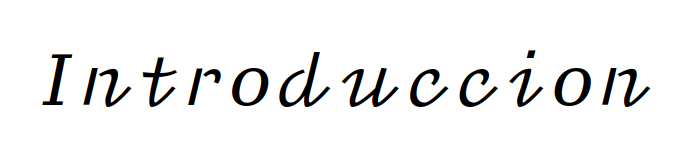
\includegraphics[width=\textwidth]{./Imagenes/T1}
    \end{subfigure}
  \end{figure}
\end{frame}

\section{Introducción (Revisitado).}
%%%%%%%%%%%%%%%%%%% Pruebas
\begin{frame}{Introducción}{Historia...}
	\justifying
        Los \underline{relojes vectoriales} son un tipo de
        reloj lógico propuesto de manera independiente por
        \textit{Colin J. Fidge} y \textit{Friedemann Mattern}
        en 1988.
        
        \begin{center}
          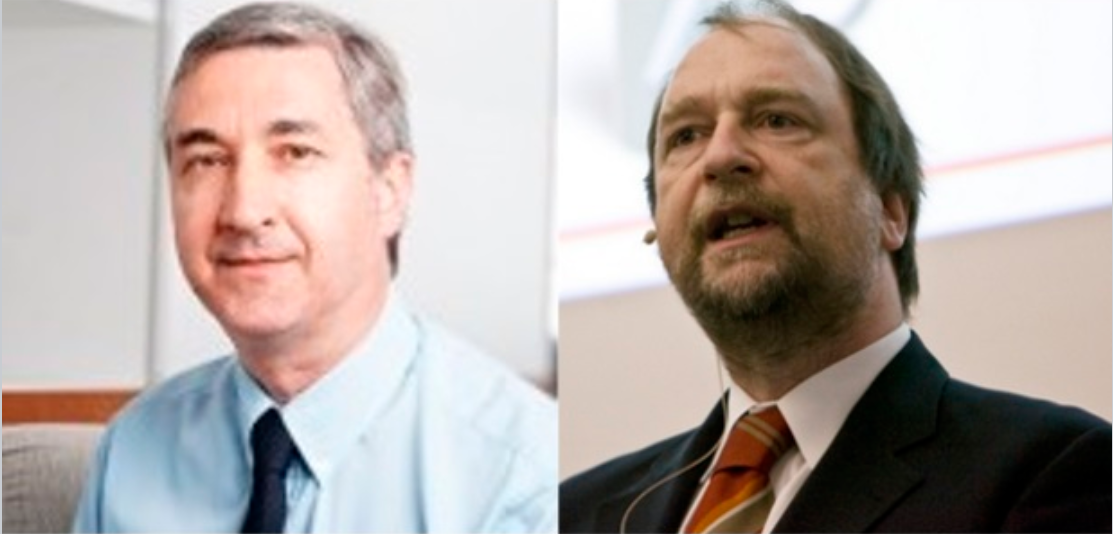
\includegraphics[height = 2cm]{./Imagenes/FidgeAndMattern.png}
        \end{center}
        
        Esta técnica consiste en un mapeo entre eventos en una
        historia distribuida y vectores enteros.
\end{frame}


\subsection{Tiempo Vectorial.}
%%%%%%%%%%%%%%%%%%% Especificación:
\begin{frame}[fragile]{Definiciones:}{Vector Tiempo.}
  \justifying
  \textbf{Sistema Vectorial de Relojes.} Es un mecanismo
  capaz de caracterizar estados locales (en adelante, eventos)
  en un sistema distribuido, asociando un valor vectorial
  a cada estado.\\[0.3cm]
  %  Esto nos permite saber que relación hay entre estos estados.
  
  \textbf{Tiempo Vectorial.} Es la noción de tiempo capturada
  por los relojes vectoriales.\\[0.3cm]

  \textbf{Caracterización Formal del Tiempo Vectorial.} Sea
  \code{date(e)} la caracterización asociada a un evento \code{e},
  de tal manera que se cumple:
  \begin{enumerate}
  \item $\forall_{e_1, e_2}:\left(e_1 \rightarrow e_2\right)
    \Leftrightarrow \code{date($e_1$)} < \code{date($e_2$)}$.
  \item $\forall_{e_1, e_2}: \left(e_1\ ||\ e_2\right) \Leftrightarrow
    \code{date($e_1$)}\ ||\ \code{date($e_2$)}$.
  \end{enumerate}
  \begin{figure}
    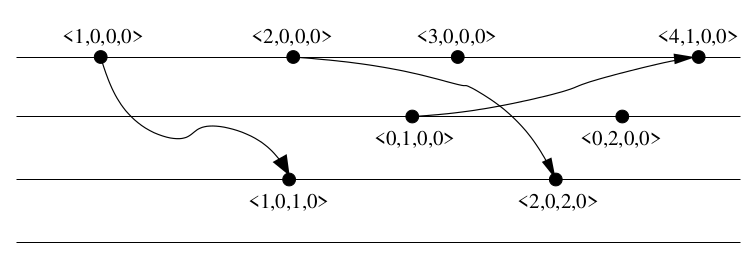
\includegraphics[height = 2.5cm]{./Imagenes/RelojVectorialSimple.png}
    \caption{Reloj Vectorial con tiempos locales.}
  \end{figure}
\end{frame}


\subsection{Relojes Vectoriales.}
%%%%%%%%%%%%%%%%%%% Especificación:
\begin{frame}[fragile]{Definiciones:}{Reloj Vectorial.}
    \justifying
    \textbf{Reloj Vectorial.} La implementación del tiempo
    vectorial requiere que cada proceso, en el sistema,
    mantenga un vector de enteros positivos $Vc_i[1, \dotsm, n]$
    con valores inicialmente $[0, \dotsm, 0]$. Este vector
    debe cumplir con
    \begin{enumerate}
    \item $Vc_i[i]$ cuenta el número de eventos producidos por
      $p_i$.
    \item $Vc_i[j]$, $j \not= i$, nos dice cuántos eventos conoce
      $p_i$ producido por $p_j$.
    \end{enumerate}
    De manera formal, sea $e$ un evento producido por $p_i$,
    tenemos que
    \[Vc_i[k] = \left|\{f | (f \text{ se produjo por } p_k) \land
    (f \rightarrow e)\}\right| + 1(k, i).\]
\end{frame}


\def\beamer@mytheme@style{green}

\subsection{Algoritmo.}
%%%%%%%%%%%%%%%%%%% Especificación:
\begin{frame}{Reloj Vectorial:}{Algoritmo.}
  \justifying
  \textbf{Una primera aproximación.} Inicialmente
  todos los procesos disponen de un vector con
  entradas igual al número total de procesos, este
  vector debe estar inicializado en $0$ para cada
  entrada. A continuación se describe el algoritmo:
  \begin{itemize}
  \item[$\blacktriangleright$] Si $p_i$ produce un evento, entonces:
    \begin{enumerate}
    \item[(1)] $Vc_i[i] \leftarrow Vc_i[i] + 1$;
    \item[(2)] Produce un evento $e$ caracterizado por $Vc_i[1, \dotsm, n]$.
    \end{enumerate}
  \item[$\blacktriangleright$] Cuando $p_i$ envia un mensaje a $p_j$, entonces:
    \begin{enumerate}
    \item[(3)] $Vc_i[i] \leftarrow Vc_i[i] + 1$;
    \item[(4)] \code{send(\textlangle msj, $Vc_i$[1, $\dotsm$, n] \textrangle)} a $p_j$.
    \end{enumerate}
  \item[$\blacktriangleright$] Cuando $p_j$ recibe un mensaje, entonces:
    \begin{enumerate}
    \item[(3)] $Vc_j[j] \leftarrow Vc_j[j] + 1$;
    \item[(4)] $Vc_j[1, \dotsm, n] \leftarrow \forall_{k \in [1, \dotsm, n]}
      \code{max}(Vc_i[k], Vc_j[k])$.
    \end{enumerate}
  \end{itemize}
\end{frame}
 % Algoritmo.
%%%%%%%%%%%%%%%%%%% Especificación:
\begin{frame}{Algoritmo:}{Propagación del tiempo vectorial.}
  \justifying
  \textbf{Notación:} Para, cualesquiera, dos vectores $Vc_1$
  y $Vc_2$ del tamaño $n$. Tenemos que
  \begin{itemize}
  \item[$\blacktriangleright$] $Vc_1 \leq Vc2 =_{def.}
    \left(\forall_{k \in \{1, \dotsm, n\}} : Vc_1[k] \leq Vc_2[k]\right)$;
  \item[$\blacktriangleright$] $Vc_1 < Vc2 =_{def.}
    \left(Vc_1[k] \leq Vc_2[k]\right) \land  \left(Vc_1[k] \not= Vc_2[k]\right)$;
  \item[$\blacktriangleright$] $Vc_1 || Vc_2 =_{def} \neg (Vc_1 \leq Vc_2) \land
    \neg (Vc_2 \leq Vc_1)$.
  \end{itemize}
  \begin{figure}
    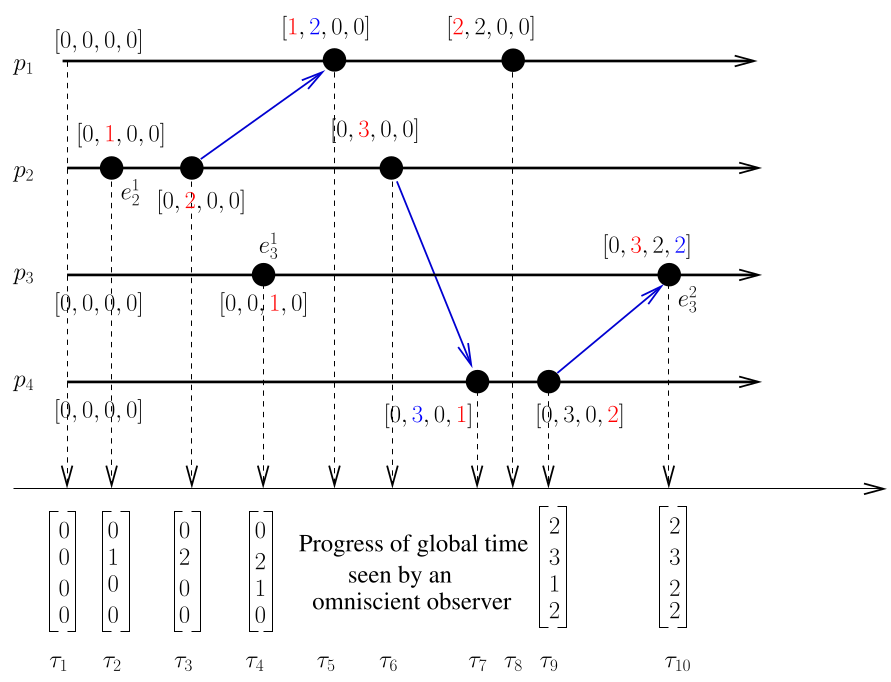
\includegraphics[height = 4.5cm]{./Imagenes/RelojVectorialCompuesto.png}
    \caption{Ejemplo de propagación en un reloj Vectorial.}
  \end{figure}
\end{frame}
 % Propagación del tiempo vectorial.
%%%%%%%%%%%%%%%%%%% Especificación:
\begin{frame}[fragile]{Algoritmo:}{Propiedades.}
  \justifying
  \textbf{Def.} Sea $e.Vc$ el vector asociado al evento $e$.\\[0.3cm]
  
  \textbf{Teo 1.} Por el algoritmo mencionado tenemos que, para cualesquiera
  $e_1$ y $e_2$ distintos tenemos que
  \begin{enumerate}
  \item[$a$)] $\left(e_1 \rightarrow e_2\right) \Leftrightarrow \left(e_1.Vc < e_2.Vc\right)$;
  \item[$b$)] $\left(e_1 || e_2\right) \Leftrightarrow \left(e_1.Vc || e_2.Vc\right)$.
  \end{enumerate}
  
  \textbf{Cor 1.} Dadas dos caracterizaciones a eventos (fechas), determinar si estos
  eventos están relacionados o no, puede requerir hasta $n$ comparaciones de enteros.
  \\[0.3cm]
  
  \textbf{Teo 2.} Sean dos eventos $e_1$ y $e_2$ con tuplas $\langle e_1.Vc, i \rangle$
  y $\langle e_2.Vc, j\rangle$ de manera respectiva y $i \not= j$. Entonces
  \begin{enumerate}
  \item[$a$)] $\left(e_1 \rightarrow e_2\right) \Leftrightarrow
    \left(e_1.Vc[i] \leq e_2.Vc[i]\right)$;
  \item[$b$)] $\left(e_1 || e_2\right) \Leftrightarrow
    \left((e_1.Vc[i] > e_2.Vc[i]) \land (e_2.Vc[j] > e_1.Vc[j])\right)$.
  \end{enumerate}
\end{frame}
 % Propiedades. 
%%%%%%%%%%%%%%%%%%% Especificación:
\begin{frame}{Algoritmo:}{Reducción de costo en la comparación de dos vectores.}
  \justifying
  \textbf{Mejora en la complejidad en tiempo.} Hasta el momento la complejidad
  en tiempo para combinar $2$ eventos nos toma $\mathcal{O}(n)$, con $n$ el
  número de procesos en el sistema.\\[0.3cm]

  Por el \textit{Teo. 2}, sabemos que basta con verificar dos entradas para
  saber como es un evento respecto al otro. Así, basta comparar dos entradas
  para combinar la caracterización de $2$ eventos esto nos toma $\mathcal{O}(1)$.
\end{frame}
 % Reducción de costo en la comparación de dos vectores.
%%%%%%%%%%%%%%%%%%%% Especificación:
\begin{frame}[fragile]{Algoritmo:}{Relación del tiempo vectorial y estados globales.}
  \justifying
  Consideremos 
\end{frame}
 % Relación del tiempo vectorial y estados globales.

\subsection{Desventajas.}
%%%%%%%%%%%%%%%%%%% Especificación:
\begin{frame}[fragile]{Relojes Vectoriales:}{Desventajas.}
  Esta mejora a los relojes lógicos de Lamport tiene un problema
  de implementación, que en un momento será más evidente. 

  \setblockstyle{native} % Default behavior, optional line.
  \begin{center}
    \begin{minipage}[b]{0.5\textwidth}
      \begin{exampleblock}{Desventaja}
        Esta desventaja es que cada proceso tiene que cargar con espacio
        igual al número de procesos en el sistema y cada intercambio
        entre eventos es de este tamaño.
      \end{exampleblock}    
    \end{minipage}
  \end{center}
\end{frame}
  % Desventajas.

% The [plain] causes the headlines, footlines, and sidebars 
% to be suppressed. Useful for showing large pictures

% TODO. Sin implementar.
%%%%%%%%%%%%%%%%%%%%%%%%%%%%%%%% Aplicación:
\begin{frame}[plain]
  \begin{figure}
    \centering
    \begin{subfigure}[b]{0.6\textwidth}
      
\includegraphics[width=\textwidth]{./Imagenes/T2}
    \end{subfigure}
  \end{figure}
\end{frame}

\section{Aplicaciones.}
\subsection{El caso DynamoDB.}
%%%%%%%%%%%%%%%%% Nat:
% Solo es el orden, cambia lo que quieras (títulos). Perdón.
%----------------------------------------------------------
\subsection{Relojes vectoriales dinámicos.}   %%%%%%%%%%%%%%%%%%%% Nat, aquí.  %%%%%%%%%%%%%%%%%%%%
%%%%%%%%%%%%%%%%%%% Especificación:
\begin{frame}[fragile]{Aplicación:}{Relojes vectoriales dinamicos}
    \justifying
    A menudo el número de procesos participando en un computo distribuido no es constante, por lo que los relojes debe ser capaces de crecer.
    
    %Para alcanzar esta flexibilidad el vector de reloj es una matriz de dos columnas, variable en su número de filas, que proporciona un mapeo simple de la ID de un proceso al valor de reloj asociado (escalar).

    El tamaño del vector está limitado por dos veces el número de procesos de los que el proceso de mantenimiento ha recibido (directa o indirectamente) valores de reloj.
    
    Cada proceso $p_i$ mantiene su propio reloj logico $C_i$ el cual es una matriz de dos columnas, variable en su número de filas, donde $C_i(e_i^x)[k,2]$, en $e_i$ almacena el valor del último reloj vectorial conocido por $p_i$ del proceso cuyo ID está en $C_i(e_i^x)[k,1]$ 

    \begin{figure}
        \centering
        \begin{subfigure}[b]{0.5\textwidth}
            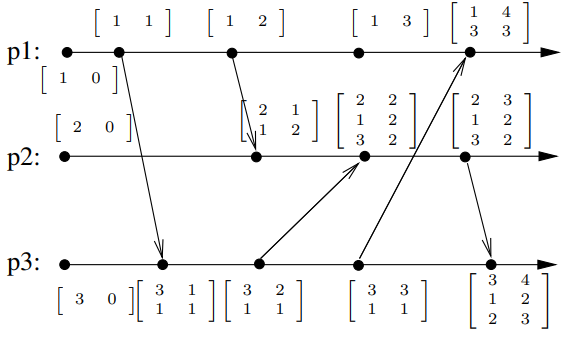
\includegraphics[width=\textwidth]{./rvd01.png}
            \caption{Ejemplo}
            \label{fig:Relojes vectoriales dinamicos}
        \end{subfigure}
        \caption{Reloj vectorial dinamico.}\label{fig:Deteccion.}
    \end{figure}    
\end{frame}
%%%%%%%%%%%%%%%%%%% Especificación:
\begin{frame}[fragile]{Aplicación:}{Relojes vectoriales dinamicos}
    \justifying
    \textbf{Las reglas para actualizar son las siguientes:} 
    
    \begin{enumerate}
        \item $\forall_{e_1, e_2}:\left(e_1 \rightarrow e_2\right)
        \Leftrightarrow \code{date($e_1$)} < \code{date($e_2$)}$.
        \item $\forall_{e_1, e_2}: \left(e_1\ ||\ e_2\right) \Leftrightarrow
        \code{date($e_1$)}\ ||\ \code{date($e_2$)}$.
        \item Al recibir $e_i^x$, entonces $\forall$
        \item d
        \item d

  \end{enumerate}
\end{frame}
\subsection{Determinando Propiedades Globales.}
%%%%%%%%%%%%%%%%%%% Especificación:
\begin{frame}[fragile]{Aplicación:}{Relojes vectoriales dinamicos}
    \justifying
    En proceso  
\end{frame}
%%%%%%%%%%%%%%%%%%% Especificación:
\begin{frame}[fragile]{Aplicación:}{Relojes vectoriales dinamicos}
    \justifying
    proceso    
\end{frame}
%%%%%%%%%%%%%%%%%%% Especificación:
\begin{frame}[fragile]{Vector Clocks in Action:}{Immediate Precessors}
    \justifying
    \textbf{El problema del seguimiento del predecesor inmediato (Immediate predecessor tracking IPT)} 
    Consiste en asociar a cada evento relevante el conjunto de eventos relevantes que son sus predecesores inmediatos.

    Además, esto se ha hecho sobre la marcha y sin añadir mensajes de control.
    
    La determinación de los predecesores inmediatos consiste en calcular la reducción transitiva (o diagrama de Hasse) del orden parcial $\widehat{R}=(R,\xrightarrow[]{re})$. 

    \justifying
    \begin{figure}
        \begin{subfigure}[b]{\textwidth}
            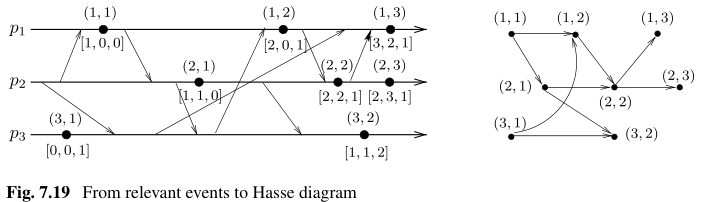
\includegraphics[scale=0.7]{Imagenes/eventosRelevantes03.png}
            \label{fig:ejemplo2}
        \end{subfigure}
    \end{figure}

\end{frame}
%%%%%%%%%%%%%%%%%%% Especificación:
\begin{frame}[fragile]{Vector Clocks in Action:}{Immediate Precessors}
    \justifying
    \textbf{Un algoritmo que resuelve el problema IPT: variables locales}
    %El k-ésimo evento relevante en el proceso pk se identifica inequívocamente por el par (k,vck), donde vck es el valor de vck[k] cuando pk ha producido este evento.
    \begin{figure}
        \centering
        \begin{subfigure}[b]{\textwidth}
            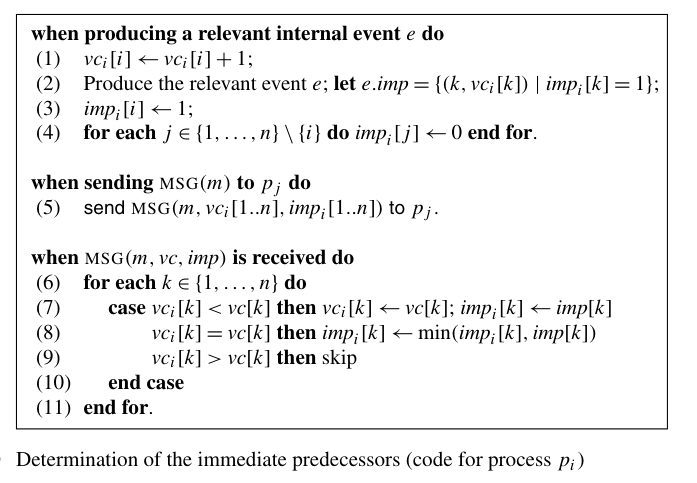
\includegraphics[scale=0.7]{Imagenes/algoIPT.png}
            \label{fig:ejemplo1}
        \end{subfigure}
    \end{figure}


\end{frame}
%----------------------------------------------------------
\subsection{Detección de una conjunción de predicados locales estables.}
%%%%%%%%%%%%%%%% Conjunción de predicados estables.
\begin{frame}[fragile]{Aplicación:}{Detección de conjunciones de predicados estables.}
  \justifying
  \textbf{Def.} Un predicado es local para $p_i$ \textit{\textbf{Sii}}
  se encuentra en variables de $p_i$ solamente.
  
  \textbf{Def.} El predicado $LP_i$ es estable \textit{\textbf{Sii}}
  en cuanto se vuelva verdadero, este permanece así siempre.
  
  \textbf{Notación:} $\sigma_i \models LP_i$. Indica que el estado local $\sigma_i$
  de $p_i$ satisface el predicado $LP_i$.
  
  \textbf{Def.} Sea $\{p_1, \dotsm, p_n\}$ un sistema distribuido y $LP_1, \dotsm, LP_n$ $n$
  predicados locales, uno por proceso (con su respectivo proceso). Un \textit{estado global
  consistente} $\sum = (\sigma_1, \dotsm, \sigma_n)$ satisface el predicado global
  $LP_1 \land \dotsm \land LP_n$ denotado por
  \[\sum \models \bigwedge_i LP_i\]
  siempre que $\bigwedge_i (\sigma_i \models LP_i)$.
  \setblockstyle{native} % Default behavior, optional line.
  \begin{center}
    \begin{minipage}[b]{0.5\textwidth}
      \begin{exampleblock}{Problema.}
        \justifying
        Detectemos sobre la \textit{historia} del sistema, y sin utilizar controles de mensajes
        adicionales, el primer estado global consistente $\Sigma$ que satisface una conjunción
        de predicados locales estables.
      \end{exampleblock}    
    \end{minipage}
  \end{center}
\end{frame}

%%%%%%%%%%%%%%%% Conjunción de predicados estables. Solución.
\begin{frame}[fragile]{Aplicación:}{Solución.}
  \justifying
\begin{figure}
    \centering
    \begin{subfigure}[b]{0.5\textwidth}
        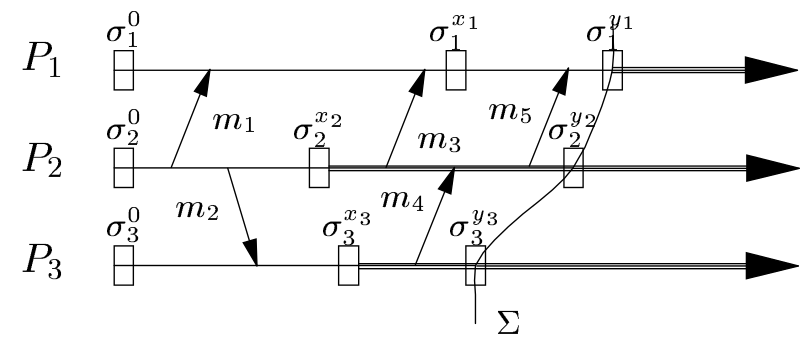
\includegraphics[width=\textwidth]{./Ejemplo1}
        \caption{Ejemplo 1.}
        \label{fig:ejemplo1}
    \end{subfigure}
    ~ %add desired spacing between images, e. g. ~, \quad, \qquad, \hfill etc. 
      %(or a blank line to force the subfigure onto a new line)
    \begin{subfigure}[b]{0.5\textwidth}
        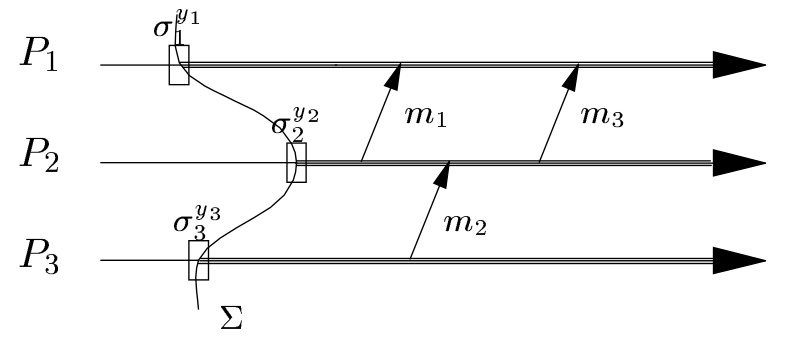
\includegraphics[width=\textwidth]{./Ejemplo2}
        \caption{Ejemplo 2.}
        \label{fig:ejemplo2}
    \end{subfigure}
    \caption{Detección de una conjunción local estable.}\label{fig:Deteccion.}
\end{figure}
\end{frame}

\subsection{Un problema de conjuntos: Conjuntos Posibles e Imposibles.}
%%%%%%%%%%%%%%%% Conjuntos Imposibles.
\begin{frame}[fragile]{Conjuntos Imposibles:}{Problema.}
  \justifying
  El problema de los \textit{conjuntos imposibles} establece:
  \begin{center}
    \textit{Dado un conjunto con n etiquetas vectoriales de k entradas cada una, decidir si
    es posible o no.}
  \end{center}

  \textbf{Ejemplo:}
  \begin{figure}
    \centering
    \begin{subfigure}[b]{0.3\textwidth}
      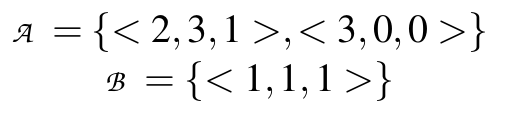
\includegraphics[width=\textwidth]{./Imagenes/Conjuntos}
        \caption{Conjuntos.}
        \label{fig:Conjuntos.}
    \end{subfigure}
    ~ %add desired spacing between images, e. g. ~, \quad, \qquad, \hfill etc. 
      %(or a blank line to force the subfigure onto a new line)
    \begin{subfigure}[b]{0.7\textwidth}
        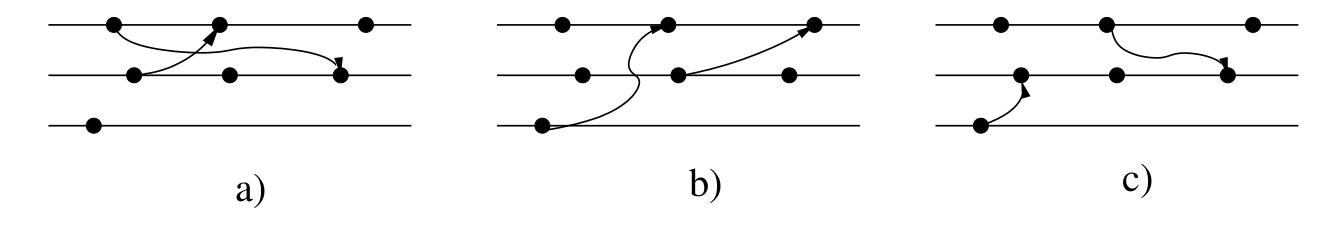
\includegraphics[width=\textwidth]{./Imagenes/Historia}
        \caption{Historias.}
        \label{fig:Historias.}
    \end{subfigure}
    \caption{Detectando conjuntos.}\label{fig:ConjuntosImposibles.}
  \end{figure}
\end{frame}


%%%%%%%%%%%%%%%%%%%%%%%%%%%%%%%% Introducción:
\begin{frame}[plain]
  \begin{figure}
    \centering
    \begin{subfigure}[b]{0.6\textwidth}
      
\includegraphics[width=\textwidth]{./Imagenes/T3}
    \end{subfigure}
  \end{figure}
\end{frame}

%%%%%%%%%%%%%% Bloom: extra.
\section{Relojes de Bloom.}
\subsection{Filtro Bloom.}
%%%%%%%%%%%%%%%% Relojes Bloom.
\begin{frame}[fragile]{Relojes Bloom:}{Filtro Bloom.}
  \justifying
  \textbf{Def.} El \textit{filtro Bloom} es una estructura de datos,
  probabilística, eficiente en espacio diseñada para verificar rápidamente
  si un elemento esta contenido en conjunto.\newline

  \textbf{Algoritmo.}
  \begin{enumerate}
  \item Definir $k$ funciones \textit{HASH} independientes.
  \item Definir un arreglo de \code{bits} con $m$ \code{bits},
    todos inicialmente igual a $0$.
  \item Para agregar un elemento al \textit{filtro bloom}, hacer
    \begin{enumerate}
    \item Pasamos el elemento, digamos $x$, por las $k$ \textit{funciones
      hash}.
    \item Cada hash apunta a un índice en el arreglo de \code{bits}
    \item La posición a la que se apunte cambia de $0$ a $1$.
    \end{enumerate}
  \end{enumerate}

  \begin{figure}
    \centering
    \begin{subfigure}[b]{0.5\textwidth}
      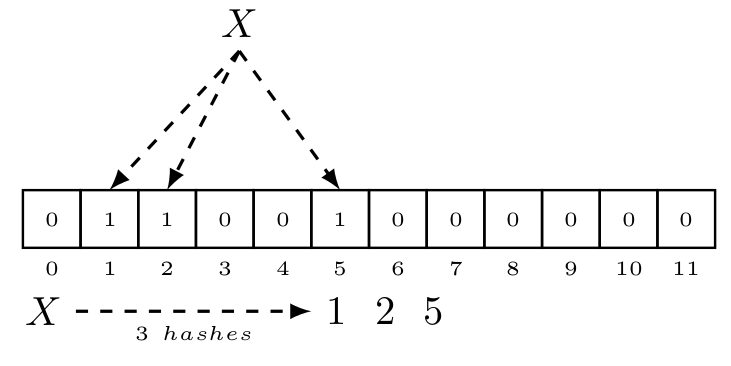
\includegraphics[width=\textwidth]{./Imagenes/Hash01}
      \caption{Inserción al filtro.}
      \label{fig:Ejemplo de Hash(X).}
    \end{subfigure}
  \end{figure}
\end{frame}

%%%%%%%%%%%%%%%% Relojes Bloom.
\begin{frame}[fragile]{Relojes Bloom:}{Filtro Bloom. Falsos positivos.}
  \justifying
  ¿Será cierto qué todos los elementos para los cuales
  las \textit{hash-funciones} nos regresen valores que en
  el \textit{bloom-filtro}  tienen asigando $1$,
  son valores que han sido introducidos al filtro?
  \begin{figure}
    \centering
    \begin{subfigure}[b]{0.5\textwidth}
      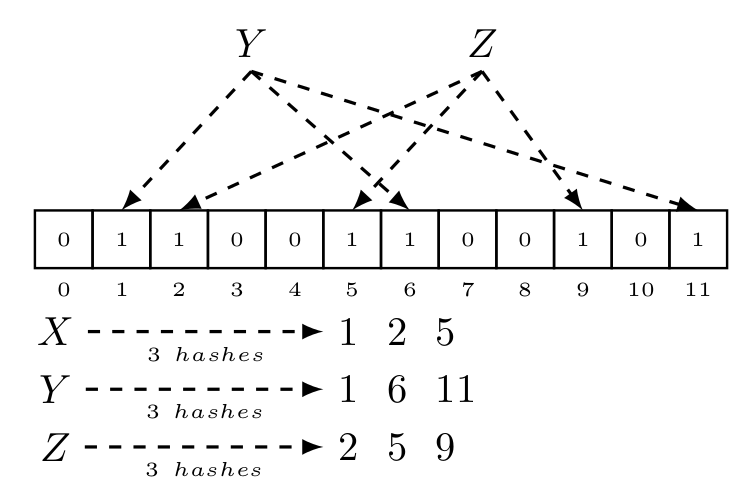
\includegraphics[width=\textwidth]{./Imagenes/FalsosPositivos}
      \caption{Falsos Positivos.}
      \label{fig:Ejemplo de un Falso Positivo.}
    \end{subfigure}
  \end{figure}
  ¿Qué podemos hacer? ...
\end{frame}


%%%%%%%%%%%%%%%% Relojes Bloom.
\begin{frame}[fragile]{Relojes Bloom:}{Filtro Bloom. Mejoras.}
  \justifying
  ¿Qué podemos hacer? ...\newline
  Podemos controlar la tasa de falsos positivos ajustando:
  \begin{enumerate}
  \item El tamaño del \textit{bloom-filtro} ($m$).
  \item El número de elementos insertados en el filtro ($n$).
  \item El número de \textit{hash-funciones} ($k$) utilizadas en la codificación.
  \end{enumerate}
  y por medio de la ecuación:
  \[\left(1 - \left(1 - \frac{1}{m}\right)^{kn}\right)^k\]
  \textbf{Idea Intuitiva:}
  \begin{itemize}
  \item $1 - \frac{1}{m}$ es la probabilidad de tener un \code{bit} en
    el filtro que no este establecido como $1$ por alguna determinada
    función.
  \item $\left(1 - \frac{1}{m}\right)^k$ es la probabilidad de que un bit
    en particular no se establezca en uno, dado que $k$ hashes pueden
    señalarlo potencialmente.
  \item $\left(1 - \frac{1}{m}\right)^{kn}$ es la probabilidad de que un
    bit en particular siga siendo cero después de $n$ elementos.
  \item $\left(1 - \left(1 - \frac{1}{m}\right)^{kn}\right)^k$ es la probabilidad
    de que $k$ índices sean $1$ después de insertar n elementos, también
    conocido como tasa de falsos positivos.
  \end{itemize}
\end{frame}

\subsection{Algoritmo.}
%%%%%%%%%%%%%%%% Relojes Bloom.
\begin{frame}[fragile]{Relojes Bloom:}{Filtro Bloom. Mejoras.}
  \justifying
  ¿Qué podemos hacer? ...\newline
  Podemos usar una variante de \textit{bloom-filtros} con conteo
  de entradas, como se muestra en el siguiente ejemplo:
    \begin{figure}
    \centering
    \begin{subfigure}[b]{0.5\textwidth}
      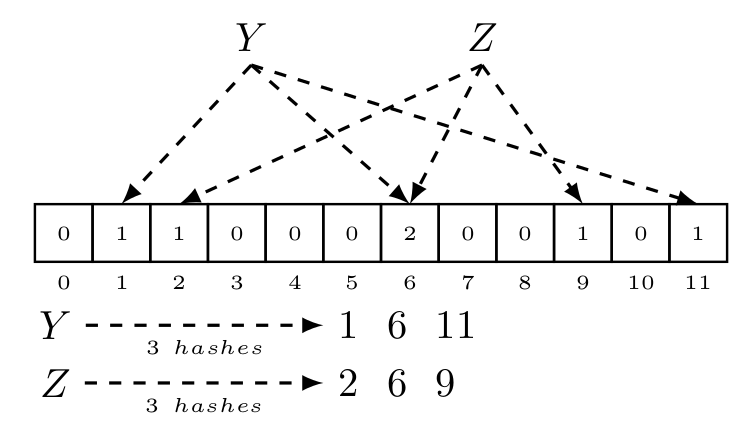
\includegraphics[width=\textwidth]{./Imagenes/CountingBloomClock}
      \caption{Filtro de Bloom tipo contador.}
      \label{fig:Ejemplo de un CountingBloomClock.}
    \end{subfigure}
  \end{figure}
\end{frame}

%%%%%%%%%%%%%%%% Relojes Bloom.
\begin{frame}[fragile]{Relojes Bloom:}{Algoritmo.}
  \justifying
  A continuación se describe el algoritmo usado en la
  dispersión de tiempos:
  \begin{enumerate}
  \item Definimos el tamaño del \textit{bloom-filtro-conteo}
    $m$ y las $k$ \textit{hash-funciones}.
  \item Cada vez que un nodo tiene un evento interno, procesa ese evento
    con $k$ \textit{hash-funciones} e incrementa su filtro. Luego envía
    ese filtro de floración a todos los demás nodos.
  \item Cada vez que un nodo recibe un evento, actualiza su filtro
    tomando el valor máximo de su filtro y el filtro receptor.
  \end{enumerate}
  \textbf{Ejemplo:}
      \begin{figure}
    \centering
    \begin{subfigure}[b]{0.45\textwidth}
      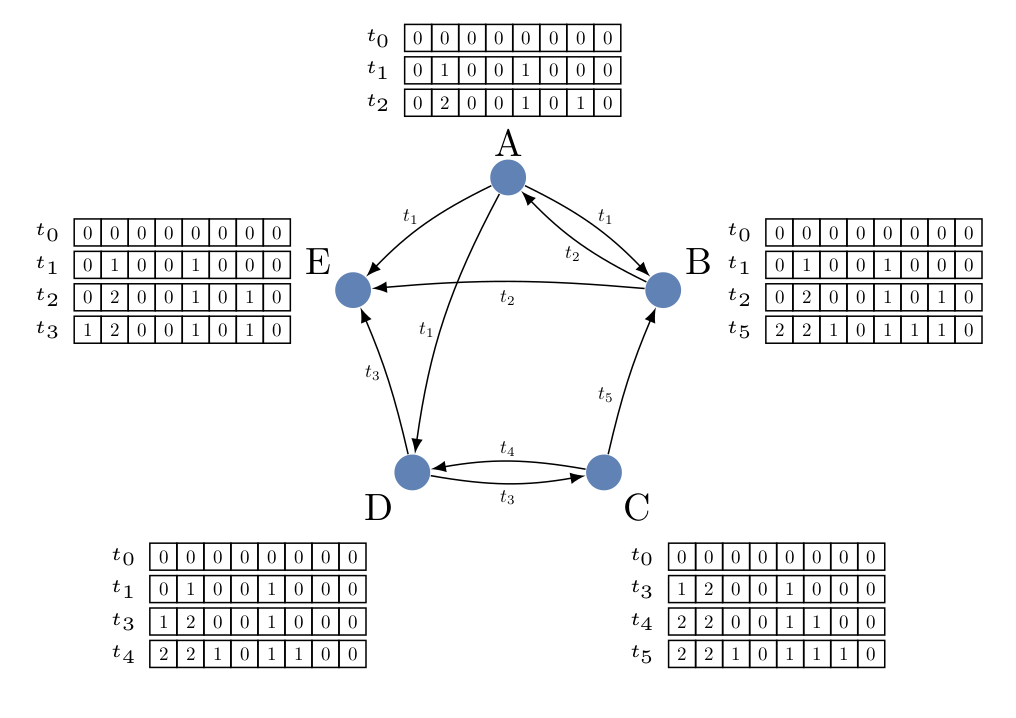
\includegraphics[width=\textwidth]{./Imagenes/RelojBloom}
      \caption{Reloj de Bloom.}
      \label{fig:Ejemplo de un CountingBloomClock.}
    \end{subfigure}
  \end{figure}
\end{frame}

\begin{frame}[fragile]{Relojes Bloom:}{Ejecución.}
  \justifying
  \textbf{Ejemplo:}
      \begin{figure}
    \centering
    \begin{subfigure}[b]{0.8\textwidth}
      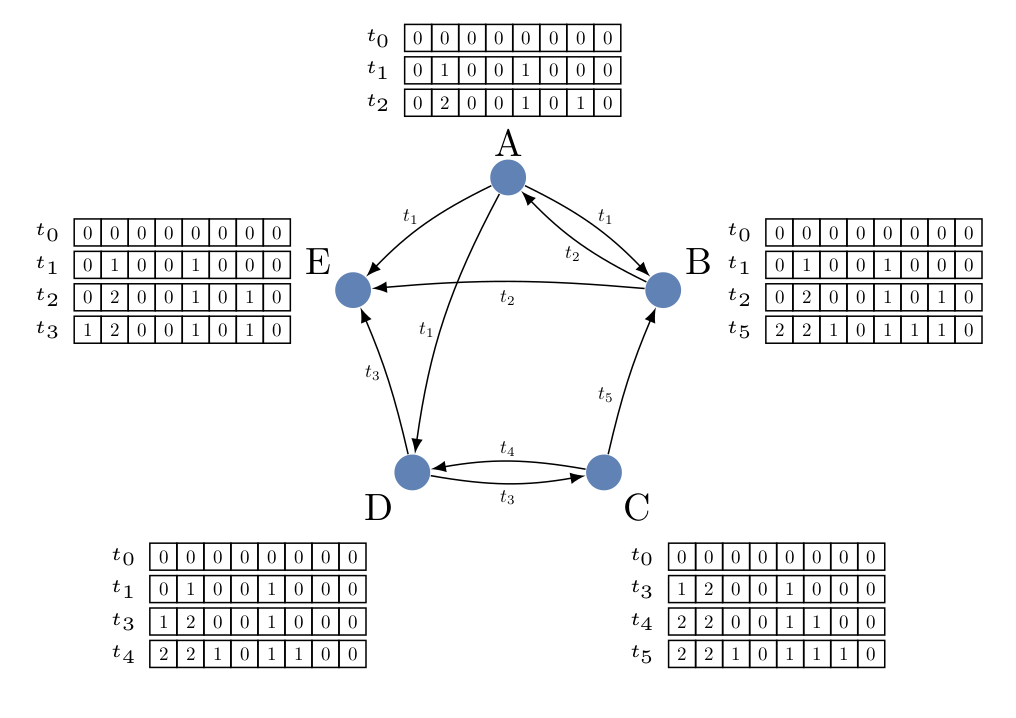
\includegraphics[width=\textwidth]{./Imagenes/RelojBloom}
      \caption{Reloj de Bloom.}
      \label{fig:Ejemplo de un CountingBloomClock.}
    \end{subfigure}
  \end{figure}
\end{frame}

%%%%%%%%%%%%%%%%%%%%%%%%%%%% Ya se terminó!!
\begin{frame}[fragile]{Relojes Bloom:}{Filtro Bloom.}
  \center ¡¡$\mathbb{AL\ FIN!!}$
  
  \begin{figure}
    \centering
    \begin{subfigure}[b]{0.4\textwidth}
      
\includegraphics[width=\textwidth]{./Imagenes/Agradecimientos}
    \end{subfigure}
    ~ %add desired spacing between images, e. g. ~, \quad, \qquad, \hfill etc. 
      %(or a blank line to force the subfigure onto a new line)
    \begin{subfigure}[b]{0.3\textwidth}
        
\includegraphics[width=\textwidth]{./Imagenes/Fin}
    \end{subfigure}
    \end{figure}
\end{frame}

\end{document}
